% 英文で執筆する場合はクラスファイルへのオプションを[T,E]としてください.
% If you want to write your paper in English, pass to [T,E] options to document class.
\documentclass[T,J]{fose} % 「コンピュータソフトウェア」用のクラスファイルは compsoft です.
\taikai{2024} % 固定です.出版委員長が毎年変更してAuthor Kitを配布してください.

\usepackage [dvipdfmx] {graphicx}

% ユーザが定義したマクロなどはここに置く.ただし学会誌のスタイルの
% 再定義は原則として避けること.

% 以下は説明のために使用したパッケージであるため,削除可能.
\usepackage{listings}
\usepackage{tabularx}
\usepackage{fancyvrb}
\usepackage{xurl}
\usepackage{cite}
\usepackage[dvipdfmx]{graphicx}
\usepackage{latexsym}
\usepackage[T1]{fontenc}
\usepackage{lmodern}
\usepackage{textcomp}
\usepackage{latexsym}
\usepackage{url}
\usepackage{longtable}
\usepackage{multirow}
%\usepackage{color}
\usepackage{xcolor}
\usepackage{colortbl}
%\usepackage[noadjust]{cite}

\newcommand{\todo}[1]{\colorbox{yellow}{{\bf TODO}:}{\color{red} {\textbf{[#1]}}}}
\newcommand{\change}[1]{\colorbox{green}{{\bf CHANGE}:}{\color{blue} {\textbf{[#1]}}}}
\newcommand{\new}[1]{\colorbox{cyan}{{\bf NEW}:}{\color{black} {\textbf{[#1]}}}}
\newcommand{\rqone}{リリースまでの期間に応じて検証/導入されるチケットの特徴に違いがあるか?}
\newcommand{\rqtwo}{リリースまでの期間に応じて優先的に検証/導入されるチケットの変化をどの程度捉えられるか?}
\newcommand{\rqthree}{\todo{rq}}

% 以下のマクロはサンプルファイル作成用のマクロです.不要であれば削除してください.
\newcommand{\foseclassfile}{fose.cls}
\newcommand{\fosestylefile}{fose.sty}


\begin{document}

% 論文のタイトル
\title{リリースまでの期間に応じて優先的に検証/導入されるコードレビューチケットの特徴分析}
% 以下の \etitle(と\@etitle)はFOSE論文フォーマット独自のマクロです.
% FOSEに投稿した論文を発展させてコンピュータソフトウェアに投稿される場合はコメントアウトしてください.
% \setetitleは奇数ページのヘッダに表示する文字列(\etitle)を設定するためのマクロです.
% タイトルが2行に渡る場合は "\\" を 使用することで任意の位置で改行をすることができます.
\setetitle{Prioritized Analysis of Reviewed or Merged Review Tickets for Each Period before Release}
%\setetitle{Long Long Long Long Long Long \\ Long Long Long Long Long \\ Long Long Long Long Long Long Long Long Long Long Long Long Paper Title}

% タイトル,著者などが複数行にわたり,論文冒頭の著者名が日本語アブストと重複して描画された場合に以下のコメントアウトを外してください.
%\longtitle

% 著者
% 和文論文の場合,姓と名の間には半角スペースを入れ,
% 複数の著者の間は全角スペースで区切る
%
\author{上中 瑞稀 伊原 彰紀
%
% ここにタイトル英訳 (英文の場合は和訳) を書く.
% 英語タイトルは論文1ページ目左下,著者らの名前・所属一覧の一番上に表示される
%
% 上記\setetitle中で改行した場合は "\etitle" を削除し,改行(\\)を入れていないタイトルを記載してください.
% \ejtitleは1ページ目左下に挿入されるタイトルとして使用されます.
% また,"\etitle"はFOSE論文フォーマット独自のマクロです.
\ejtitle{\etitle}
\shozoku{Mizuki Uenaka, Akinori Ihara}{和歌山大学}
{Wakayama University}
}

%
% 和文アブストラクト
% In English paper, content of Jabstract will be ignored. 
\Jabstract{%
オンラインコードレビューサービスを導入するOSS開発では,日々多くのコードレビューを依頼するコードレビューチケットが提出され,検証者は優先的にコードレビューするチケットを選択する.従来研究では,チケット提出時に得られる特徴に基づき優先順位づけする手法が提案されているが,コードレビューするチケットの優先順位は日々変動する.本研究では,直近のリリースまでの期間に応じて検証/導入されるコードレビューチケットの特徴の違いを分析する.また,リリースまでの期間別に優先的に検証/導入されるコードレビューチケットを予測する.ケーススタディとして,OpenStackプロジェクトを対象に分析した結果,リリースまでの期間に応じて検証/導入されるチケットの特徴には違いがあることを明らかにした.また,優先的に検証/導入されるコードレビューチケットを予測した結果,優先的に検証/導入する必要のないチケットの検出では提案手法の有用性が示された.
}
%
\maketitle \thispagestyle {empty}


%%%%%%%%%%%%%%%%%%%%%%
\section{はじめに}
%%%%%%%%%%%%%%%%%%%%%%

ソフトウェア開発において,変更提案されたソースコードの可読性や欠陥の有無を開発者が評価するコードレビューの作業は,ソフトウェアの品質維持のために重要な役割を担っている~\cite{quality1}\cite{quality2}.コードレビューでは,複数人の開発者(検証者)がソースコードを検証し,ソースコードを実装した開発者(実装者)と共にソースコード変更の妥当性について合意形成を図り,必要に応じて修正を繰り返す.

コードレビューはソフトウェア開発プロセスの一連の作業において,時間,作業量ともに高いコストを要する作業である\cite{cost}.コードレビューを効率化するため,昨今ではGitHub,Gerrit,Review Boardなどのオンラインコードレビューサービスを利用した方式(モダンコードレビュー\cite{quality1})の導入が増加している.このようなサービスではソースコードの変更提案をレビューチケットとして保存・管理する.大規模なソフトウェア開発プロジェクトでは,日々膨大なソースコードの変更提案が提出されており,検証者は変更提案の内容や緊急性を考慮しながら優先的に検証するチケットを選択している\cite{integrator}.

従来研究では,チケット提出時に得られる特徴(変更行数や変更ファイル数など)に基づき,開発者らが優先的に検証するチケットを機械学習アルゴリズムを用いて特定する手法を提案している\cite{prioritizer}\cite{review_prioritize_pineapple}.当該手法は,セキュリティに関連するようなソフトウェア利用者に悪影響を与えるソースコードの改善のように,チケット提出時期によって優先順位の変動が小さいチケットの特定に有用である.
%急を要さない不具合修正,リファクタリングの変更提案に関する
しかし,検証する優先順位が日々変動するチケットが存在する.Kononenkoらは,開発者へのインタビューにおいて,直近のリリースに導入するチケットの優先順位はリリースまでの期間によって異なることを明らかにしている\cite{release_merge}.特に,ラピッドリリースを導入しているプロジェクトでは検証を次のリリースに延期することも少なくない.従来手法は,このようなリリースまでの期間などの開発状況に応じた検証するチケットの優先順位の決定には適していない.

本研究では,直近のリリースまでの期間に応じて検証されるコードレビューチケットの特徴の違いを明らかにする.さらに,リリースまでの期間別に優先的に検証されるコードレビューチケットを予測する有効性を明らかにする.また,従来研究\cite{estimate_merge_time}ではコードレビューに要する時間はチケットの特徴に限らず,チケット提出時期にも依存するため,本研究では直近のリリースまでの期間に応じて導入されるコードレビューチケットも分析する.本研究では,コードレビューツールGerritを使用するクラウド基盤ソフトウェアOpenStackの6つのコアコンポーネントプロジェクトを対象に2つのリサーチクエスチョン (RQ) を検証する.

\noindent\textbf{RQ1: \rqone}\\
RQ1では,従来研究\cite{prioritizer}で提案されている開発者やチケットの特徴(4種類)と従来研究\cite{review1}\cite{release_merge}の知見から有用と示唆される開発者や変更内容の特徴(3種類)を特徴量として計測し,リリースまでの期間別に検証/導入されるコードレビューチケットの特徴量の違いを分析する.

\noindent\textbf{RQ2: \rqtwo}\\
RQ2では,RQ1で計測した特徴量を用いてチケットが直近のリリースに検証/導入されるか否かを予測するモデルをリリースまでの期間別に構築し,評価する.また従来研究との比較として分析対象期間を区別しないモデルによる予測結果と比較する.

以降,本論文では,\ref{sec:intro}章でOSS開発におけるコードレビュープロセスと従来研究について述べる.その後,\ref{sec:dataset}章で分析対象とするデータセットを述べ,\ref{sec:rq1},\ref{sec:rq2}章でRQ1,RQ2の分析手法および結果を述べる.そして,\ref{sec:disc}章で結果の考察および妥当性の脅威について述べ,\ref{sec:fig-tab-exp}章でまとめる.

%%%%%%%%%%%%%%%%%%%%%%
\section{ソフトウェア開発におけるコードレビュープロセス}\label{sec:intro}
%%%%%%%%%%%%%%%%%%%%%%

\subsection{コードレビュープロセス}
図\ref{fig:codereviewprocess}はコードレビュー作業の一連の流れを説明する概略図を示す.検証者は,実装者が提出したコードレビューチケットを確認し,変更提案に対して3つの判断(導入,却下,修正要求)のいずれかを決定する.導入はソースコードをリポジトリに導入し,却下はソースコードを導入することなくコードレビューチケットを閉じる.修正要求は,コードレビューチケットを提出した実装者にソースコードの改修を依頼する.検証者は,修正要求を繰り返すことで,ソフトウェアの品質を維持しつつ,不具合修正やさらなる機能拡張を行う.

コードレビューはソフトウェア開発に多大な貢献をもたらす一方で,膨大なコストがかかる作業でもある.1つのコードレビューチケットの確認に数日から数ヶ月の期間を要することもあり,1週間で平均6時間程度をコードレビューに費やすプロジェクトも多い\cite{review2}.特に,大規模なオープンソースソフトウェア (OSS) 開発では,膨大なチケットを受け付けるため,検証者は変更提案の内容や緊急性を考慮して,優先的に検証するチケットを選択している\cite{integrator}.

%-----------------------
\begin{figure}[t]
\begin{center}
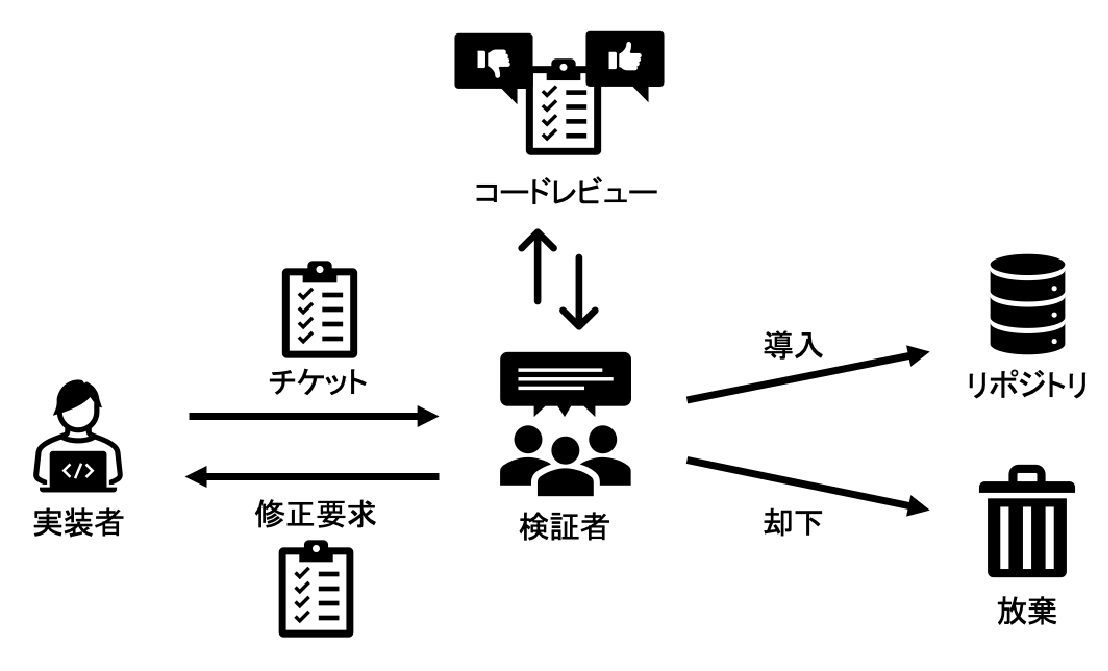
\includegraphics[width=1.0\linewidth]{Uenaka_fig/code_review_process.pdf}
\caption{コードレビュープロセス}
\label{fig:codereviewprocess}
\end{center}
\end{figure}
%-----------------------

\subsection{従来研究}

\subsubsection{チケットの優先順位付け}
Veen\cite{prioritizer}らは,OSS開発を対象にコードレビューの優先順位付け手法を提案している.従来研究では,機械学習アルゴリズムを用いて,変更内容や作成者の特徴などの14種類の特徴を説明変数とし,コードレビューチケットに翌日までに検証結果が投稿されるか否かを予測する手法を提案している.当該研究ではリリースまでの期間によって日々優先順位が変動するような変更提案のチケットに対して誤った優先順位を算出することが示唆される.そのため,本研究ではリリースまでの期間ごとに予測モデルを構築し,ベースラインと比較することでリリースまでの期間による予測精度の違いを分析する.

\subsubsection{開発者の貢献量がチケットの検証/導入判断にもたらす影響}
Bosu\cite{review1}らは,OSS開発における開発者の地位がチケットの導入に影響するのか否かを明らかにするために,OSS開発に積極的に貢献する開発者と消極的な開発者がそれぞれ作成したソースコードのレビュープロセスの違いを調査した.8つのOSSプロジェクトから導入もしくは却下と判断されたチケットのコードレビューデータを調査した結果,積極的に貢献する開発者のチケットほど,導入もしくは却下までの時間が短く,導入される確率が高いことが明らかとなった.そのため本研究では,実装者の貢献量を捉えるため,従来研究\cite{prioritizer}の特徴量である導入実績(実装者が過去に提案したチケットの導入率)だけでなく,報告実績(実装者が過去に提案したチケット数)を特徴量に加え,リリースまでの期間ごとの特徴量の違いを分析する.

\subsubsection{変更内容がチケットの検証判断にもたらす影響}
Kononenko\cite{release_merge}らは,コードレビューにかかる時間および導入判断に影響を与える要因を明らかにするためにコードレビューチケットを調査した.定性的分析として開発者へのインタビューを行った結果,レビューにかかる時間は変更内容(バグ修正,リファクタリング等)によって異なることが明らかとなった.そのため,本研究では変更内容によって検証判断が異なると考え,従来研究\cite{bug}\cite{refactoring}において利用されていた
チケットのタイトルと概要に含まれる単語に基づき,バグ修正,リファクタリング,またはその他に分類し,バグ修正確信度とリファクタリングを特徴量に加え,リリースまでの期間ごとの特徴量の違いを分析する.

\subsection{本研究の動機}
従来研究\cite{prioritizer}は,優先順位の変動が小さいコードレビューチケットの特定には有用である.しかし,提出されるチケット数に対して検証可能な開発者数のような開発リソースが少ない場合,検証/導入可能なチケット数に限りがあるため,リリースまでの期間に検証の優先順位が変化するチケットの選択には適していない.

本研究では,RQ1としてリリースまでの期間に着目し,リリースまでの期間別に検証/導入されるコードレビューチケットの特徴を分析する.RQ2では,RQ1で分析した特徴量を用いてリリースまでの期間別に,優先的に検証/導入されるコードレビューチケットを予測する.


%%%%%%%%%%%%%%%%%%%%%%%%%%%%%%%%%%%%%%%%%%
\section{分析対象データセット}\label{sec:dataset}
%%%%%%%%%%%%%%%%%%%%%%%%%%%%%%%%%%%%%%%%%%
本研究では,OpenStackプロジェクトのうち,コアコンポーネント6プロジェクト(Nova,Neutron,Cinder,Keystone,Swift,Glance)を分析対象とする.各プロジェクトの変更提案の中で,立ち上げ時から2022年9月時点で導入もしくは却下されたコードレビューチケットを収集する.具体的には,OpenStackがコードレビュー管理システムとして使用するGerrit\footnote{Gerrit: \url{https://review.opendev.org}}から,コードレビュー履歴を収集し,変更提案のチケットの特徴量を計測した.またGitHubから,各バージョンのリリース日およびリリースに導入されたチケットの特定を行った.
分析対象プロジェクトのリリース間隔が約3ヶ月であるため,本研究では各プロジェクトでリリースに導入されたコードレビューチケットの変更提案を対象とし,特にリリース直前の3ヶ月に導入されたチケット数の上位5バージョンを分析対象とする.表\ref{table:release}は分析対象とする各プロジェクトのバージョンを示す.また,長期間に渡り放置される変更提案は,短期的な優先順位の決定には関与しないため,リリース直前の6ヶ月以内に提出されたチケットを分析対象とする.

%------------------------
\begin{table*}[t]
\centering
  \caption{プロジェクトごとの対象リリースバージョン}
  \vspace{0.5zh}
  \label{table:release}
  \scalebox{0.88}{
  \begin{tabular}{l|r|l}  \hline \hline
    プロジェクト &チケット数 & \multicolumn{1}{c}{バージョン(リリース3ヶ月以内に導入されたチケット数 )}\\ \hline 
    Nova & 39,870 & 13.0.0.0b3(529),14.0.0.0b1(475),16.0.0.0b2(451),17.0.0.0b1(410),20.0.0.0rc1(392)\\ 
    Neutron & 24,467 & 7.0.0.0b1(326),8.0.0.0b1(400),9.0.0.0b1(296),11.0.0.0b1(286),16.0.0.0b1(186)\\ 
    Cinder & 17,155 & 8.0.0.0b1(249),8.0.0.0rc1(249),9.0.0.0b2(249),11.0.0.0b2(249),12.0.0.0b2(235)\\ 
    Keystone & 10,764 & 8.0.0a0(182),9.0.0.0b3(211),10.0.0.0b2(220),11.0.0.0b1(167),15.0.0.0rc1(165)\\ 
    Swift & 8,737 & 1.9.2(180),2.4.0(154),2.7.0(117),2.17.0(105),2.27.0(101)\\ 
    Glance & 6,248 & 11.0.0a0(70),12.0.0.0b1(83),12.0.0.0b3(72),13.0.0.0b1(64),17.0.0.0b1(73)\\ \hline
  \end{tabular}
  }
\end{table*}
%------------------------


%%%%%%%%%%%%%%%%%%%%%%
\section{RQ1: \rqone}\label{sec:rq1}
%%%%%%%%%%%%%%%%%%%%%%

\subsection{分析手法}

\subsubsection{コードレビューチケットの分類}
本研究では,リリースまでの3ヶ月の期間内に検証/導入されるコードレビューチケットの特徴量の違いを明らかにする.具体的には,各プロジェクトのリリース間隔が約3ヶ月(12週間)であるため,リリース直前の12週間を図\ref{fig:labeling}に示すように12週前から8週前までを初期,8週前から4週前までを中期,4週前からリリースまでを終期として4週間ずつの3期間に分割し,それぞれの期間において優先的に検証されたチケットの特徴量の違い(RQ1-1),および優先的に導入されたチケットの特徴量の違い(RQ1-2)をそれぞれ分析する.

\textbf{(RQ1-1 検証)} 本研究では各期間において,従来研究\cite{prioritizer}と同様に,検証者からのコメントや評価が投稿されれば優先的に検証されるチケットと捉え「検証開始済み」に分類し,チケットの提出から検証を開始するまでは「非検証」に分類する.本研究では,時期に応じて優先的に検証を要すると判断されるチケットの特徴を明らかにするため,検証が開始されたチケットは,次の期間以降から分析対象外とする.
図\ref{fig:labeling}のチケットを例に説明すると,対象チケットは初期に提出されてはいるが,当該時期にまだ検証されていないため「非検証」に分類する.また,中期に検証者からのコメントや評価が投稿されたため「検証開始済み」に分類し,終期以降は分析対象外とする.

\textbf{(RQ1-2 導入)} 本研究では各期間において,GitHubリポジトリにマージ処理されると「導入済み」に分類し,チケットの提出からリポジトリにマージ処理されるまでは「非導入」に分類する.また「導入済み」のチケットは,次の期間以降から分析対象外とする.
図\ref{fig:labeling}のチケットを例に説明すると,対象チケットは初期や中期では導入されていないため「非導入」に分類する.また,終期にマージ処理されたため「導入済み」に分類し,以降は分析対象外とする.

%-----------------------
\begin{figure}[t]
\begin{center}
\scalebox{1.3}{
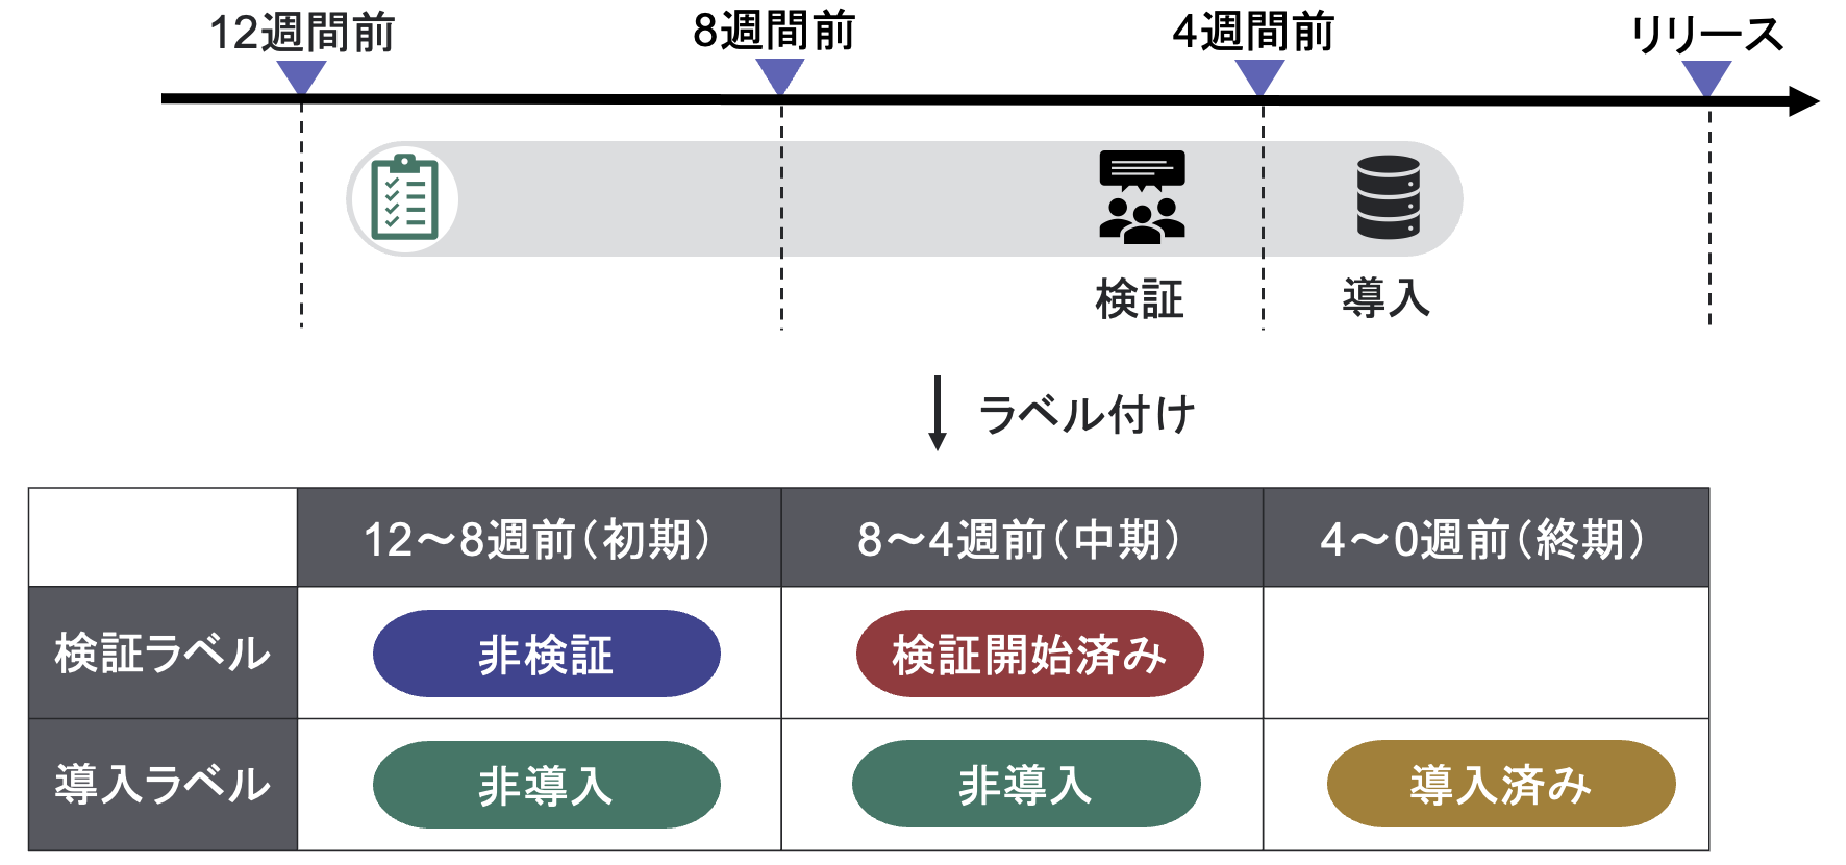
\includegraphics[width=0.8\linewidth]{Uenaka_fig/labeling.pdf}
}
\caption{チケットに対するラベル付け例}
\label{fig:labeling}
\end{center}
\end{figure}
%-----------------------


\subsubsection{レビューチケットの特徴量の計測}
本研究では,表\ref{table:metrics}に示す7種類の特徴量をリリースまでの各期間における分析対象のチケットから計測する.これらの特徴量は,従来研究に基づき決定した特徴量である.ただし,従来研究で計測していたGitHub特有の説明変数は計測対象外とする.
バグ修正確信度は,従来研究\cite{bug}において利用されていた正規表現をチケットのタイトルと概要に適用することで,チケットがバグである確度を3値に分類した特徴量である.
なお,本研究では報告実績等の時系列によって値が変化する特徴量は,同一の変更提案でもリリースまでの期間別に再計測する.

%-----------------------
\begin{table}[t]
  \caption{RQ1の分析に用いる7種類の特徴量}
  \label{table:metrics}
  \centering
  \vspace{0.5zh}
    \scalebox{0.65}{
  \begin{tabular}{l|l|l}
    \hline \hline
    \multicolumn{1}{c|}{特徴量}  & \multicolumn{1}{c|}{説明}  & \multicolumn{1}{c}{従来研究}  \\
    \hline
    報告実績  & 実装者が過去に提案したチケット数  & \cite{review1} \\
    導入実績  & 実装者が過去に提案したチケットの導入率  & \cite{review1},\cite{prioritizer} \\
    追加行数  &  チケットで追加されている変更行数  & \cite{prioritizer},\cite{diff} \\
    削除行数  & チケットで削除されている変更行数  & \cite{prioritizer},\cite{diff}  \\
    テストコード含有  & 変更ファイルにテストが含まれているか  & \cite{prioritizer} \\
    バグ修正確信度  &  バグ修正の変更提案である確度  & \cite{bug},\cite{release_merge} \\
    リファクタリング  & リファクタリングの変更提案か否か  & \cite{refactoring},\cite{release_merge} \\
    \hline
  \end{tabular}
  }
\end{table}
%-----------------------

\subsubsection{レビューチケットの特徴量の比較}
初期,中期,終期の3つの期間における検証/導入されるコードレビューチケットの特徴量を分析する.具体的には,リリースまでのそれぞれの期間において,未検証チケットと検証開始済みチケット,また導入チケットと非導入チケットに関する特徴量の違いをそれぞれマンホイットニーのU検定を用いて統計的有意差を確認する.

%--------------------
\begin{table*}[t]
\caption{RQ1-1:検証される変更提案と検証されない変更提案の特徴量の検定結果\\(Nova(No),Neutron(Ne),Cinder(C),Keystone(K),Swift(S),Glance(G))}
\label{table:review_notreview_prepare}
\centering
\vspace{0.5zh}
\scalebox{0.76}{
\begin{tabular}{l|cccccc|cccccc|cccccc}
    \hline \hline
    \multirow{2}{*}{特徴量} & \multicolumn{6}{c|}{初期} & \multicolumn{6}{c|}{中期} & \multicolumn{6}{c}{終期} \\ \cline{2-19}
    & No & Ne & C & K & S & G & No & Ne & C & K & S & G & No & Ne & C & K & S & G \\ \hline
    導入実績 & *** & *** &  &  &  & *** & *** & *** & * & ** &  & *** & *** & *** & *** & *** &  & *** \\
    報告実績 &   &  & ** & *** &   & ** &   &   & *** & *** & * &   &  & *** &  &  &  *** &  \\
    追加行数 & *** & *** & * & *** & *** & *** & *** & *** & *** & *** & *** & *** & *** & *** & *** & *** & *** & *** \\
    削除行数 & * & *** &  &  & ** &   &  & * &   &   & *** &   &   &  & ** &  &   &  \\
    テストコード含有 & *** &  &  & *** &   &   & *** &   &   &   &   & * &  & ** & * & * &   &  \\
    バグ修正確信度 & *** & *** & *** & ** &  & *** & *** & *** & *** &  &   & ** & *** & *** & *** & * &   & *** \\
    リファクタリング &  &  &  & ** &   &  &   & * & ** &  &   &  &  &   & ** &    &   &  \\ \hline
\end{tabular}}


\vspace{2mm}
\caption{RQ1-2:導入される変更提案と導入されない変更提案の特徴量の検定結果\\(Nova(No),Neutron(Ne),Cinder(C),Keystone(K),Swift(S),Glance(G))}
\label{table:merge_notmerge_prepare}
\centering
\vspace{0.5zh}
\scalebox{0.76}{
\begin{tabular}{l|cccccc|cccccc|cccccc}
    \hline \hline
    \multirow{2}{*}{特徴量} & \multicolumn{6}{c|}{初期} & \multicolumn{6}{c|}{中期} & \multicolumn{6}{c}{終期} \\ \cline{2-19}
    & No & Ne & C & K & S & G & No & Ne & C & K & S & G & No & Ne & C & K & S & G \\ \hline
    導入実績 & *** & *** & *** & *** & *** & *** & *** & *** & *** & *** & *** & *** & *** & *** & *** & *** & *** & *** \\
    報告実績 & *** & *** & *** & *** & * & *** & *** & *** & *** & *** &   & * & *** & *** & *** & *** &  &  \\
    追加行数 & *** & *** & *** & * & *** & * & *** & *** & *** & *** & *** & *** & *** & *** & *** & *** & *** & *** \\
    削除行数 &   & ** &  &  &  &   &   &   & ** &   &   &   &   &    &   &  & * & ** \\
    テストコード含有 & *** & *** &  & *** &   & *** & *** & *** & *** & *** & * & ** & *** & *** &  & ** & ** &    \\
    バグ修正確信度 & *** & *** & *** &   &   &  *  & *** & *** & *** & *** & ** & *** & *** & *** &    & * &   & *** \\
    リファクタリング & *** &   & ** &   &  *  & ** &   &   &   &   &   & * & ** &   &   &    & ** & * \\ \hline
\end{tabular}}
\end{table*}
%--------------------

\subsection{結果}
RQ1では,リリースまでの期間(初期,中期,終期)に応じて,検証開始済み/非検証のチケットや導入済み/非導入のチケットの特徴量に対してマンホイットニーのU検定を用いることで,チケットの特徴量を比較する.結果の表では,P値が0.01未満は***,0.01〜0.05は**,0.05〜0.1は*で表記する.

\textbf{(RQ1-1 検証)} 表\ref{table:review_notreview_prepare}は,各プロジェクトの初期,中期,終期において検証されるチケットと検証されないチケットの特徴量の検定結果を示す.表\ref{table:review_notreview_prepare}の結果から,多くのプロジェクトにおいて追加行数の特徴量はいずれの期間でも検証開始済み/非検証のチケット間で統計的に有意な差があることを確認した.したがって,どの時期でも追加行数は検証判断において重要であることが示唆される.次に,導入実績はCinderプロジェクトやKeystoneプロジェクトにおいて,初期では統計的有意差を確認できなかったが,中期や終期それぞれでは統計的有意差を確認できた.
図\ref{fig:review_notreview}は,有意差を確認できたCinderプロジェクトの未検証チケットと検証開始済みチケットの導入実績の分布を示す.終期における未検証チケットと検証開始済みチケットをそれぞれ作成した開発者の導入実績(中央値の差)は,初期や中期に比べて大きく,終期には導入実績の高い開発者が作成したチケットを優先的に検証されていることが示唆される.したがって,リリースまでの期間に応じて検証されるチケットの特徴には違いがあることが示唆された.


%-----------------------
\begin{figure}[t]
\begin{center}
\scalebox{1.0}{
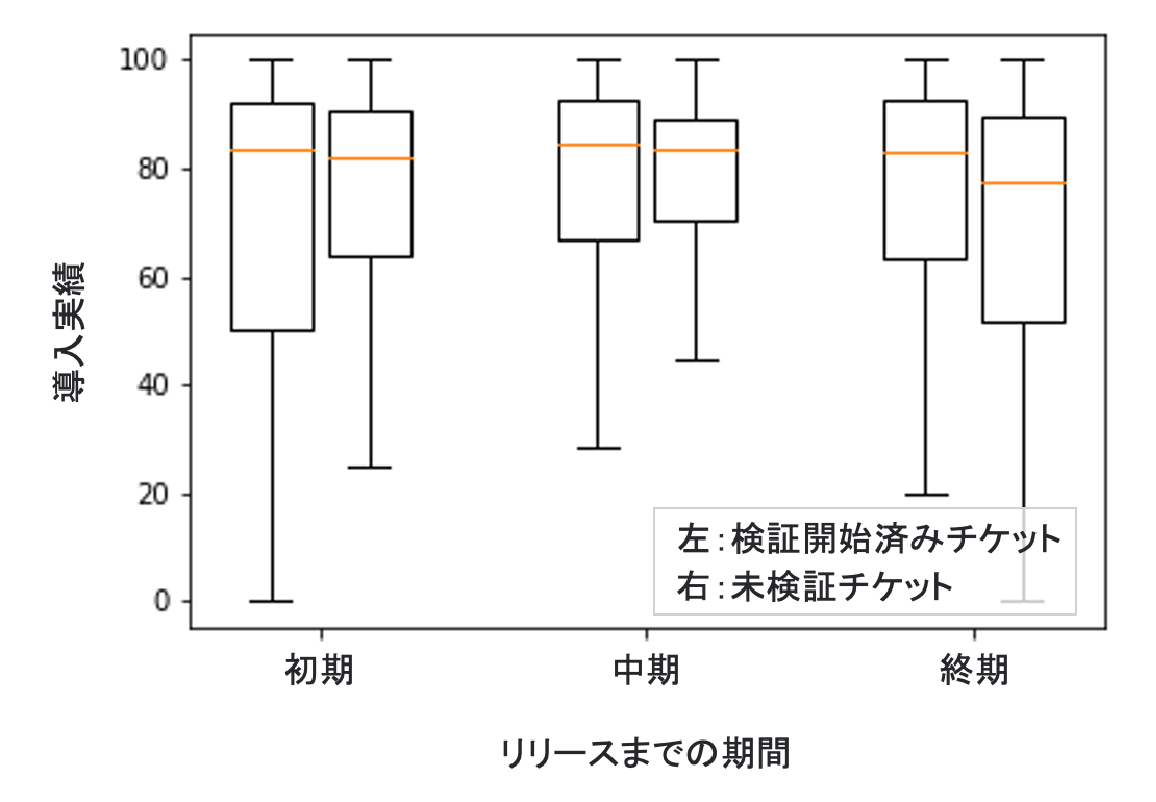
\includegraphics[width=0.8\linewidth]{Uenaka_fig/review_notreview.pdf}
}
\caption{Cinderプロジェクトにおける検証開始済み/非検証のチケットの導入実績の分布}
\label{fig:review_notreview}
\end{center}
\end{figure}
%-----------------------

%-----------------------
\begin{figure}[t]
\begin{center}
\scalebox{1.0}{
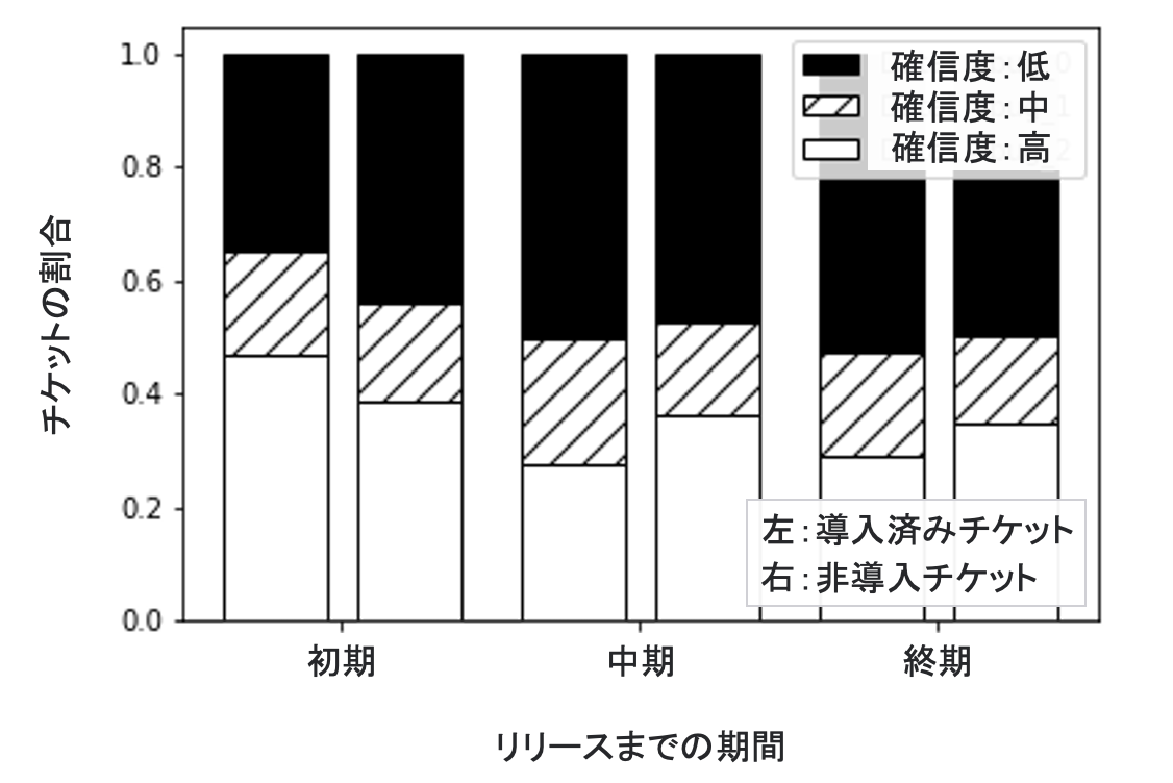
\includegraphics[width=0.8\linewidth]{Uenaka_fig/merge_notmerge.pdf}
}
\caption{Keystoneプロジェクトにおける導入済み/非導入のチケットのバグ修正確信度の分布}
\label{fig:merge_notmerge}
\end{center}
\end{figure}
%-----------------------

\textbf{(RQ1-2 導入)} 表\ref{table:merge_notmerge_prepare}は各プロジェクトの初期,中期,終期において導入されるチケットと導入されないチケットの特徴量の検定結果を示す.表\ref{table:merge_notmerge_prepare}の結果から,導入実績,追加行数の特徴量は全てのプロジェクトの全期間において,導入済み/非導入のチケット間で統計的に有意な差があった.この結果から,どの時期でも導入実績および追加行数は導入判断において重要であることが示唆される.一方,バグ修正確信度は初期や終期と比べて中期の方が統計的に有意差のあるプロジェクトが増加する.図\ref{fig:merge_notmerge}にリリースまでの期間によって有意差の変化したKeystoneプロジェクトの導入済みチケットと非導入チケットのバグ修正確信度の分布を示す.バグ修正確信度は提案がバグ修正である確度を3値に分類した特徴量であり,図\ref{fig:merge_notmerge}では黒色で示されている提案が最もバグである確度が低く,次いで斜線,白色と図\ref{fig:merge_notmerge}の積み上げ棒グラフの下部の分類ほどバグである確度が高い.この結果から,特に中期ではバグ修正確信度の低いチケットが優先的に導入されるという結果が得られた.
なお,終期も中期と同じような結果であるが,これは終期のバグ修正確信度にも導入済み/非導入のチケット間で統計的に有意な差があったためであると考えられる.したがって,リリースまでの期間に応じて導入されるチケットの特徴には違いがあることが示唆された.


%%%%%%%%%%%%%%%%%%%%%%%%%%%%%%%%%
\section{RQ2: \rqtwo}\label{sec:rq2}
%%%%%%%%%%%%%%%%%%%%%%%%%%%%%%%%%
\subsection{分析手法}

\subsubsection{予測モデルの構築}
RQ2では,直近のリリースまでに検証されるか否か,直近のリリースまでに導入されるか否かを目的変数とする2クラス分類モデル(検証予測モデル,導入予測モデル)を期間別に構築する.図\ref{fig:predict_schematic}は,予測モデルを構築するための概略図を示す.本研究では提案手法として各分析区間のデータを用いて学習および評価を行う初期モデル,中期モデル,終期モデルの3モデルを構築し,ベースライン手法として全ての期間のデータセットを用いて,それぞれの期間で学習モデルを構築し,分析区間ごとに評価を行う.具体的には,5バージョンのうち最も新しい1つをテストデータとし,残り4つを学習データとすることで各モデルを構築する.
検証予測モデルおよび導入予測モデルの構築には,それぞれ機械学習アルゴリズムであるRandom Forestsモデル\cite{randomforest}を用いる.しかし,RQ2では目的変数が不均衡なデータを扱うため,Balanced Random Forestモデル\footnote{imblearn.ensemble.BalancedRandomForestClassifier: \url{https://imbalanced-learn.org/stable/references/generated/imblearn.ensemble.BalancedRandomForestClassifier.html}}を用いる.

%-----------------------
\begin{figure}[t]
\begin{center}
\scalebox{1.25}{
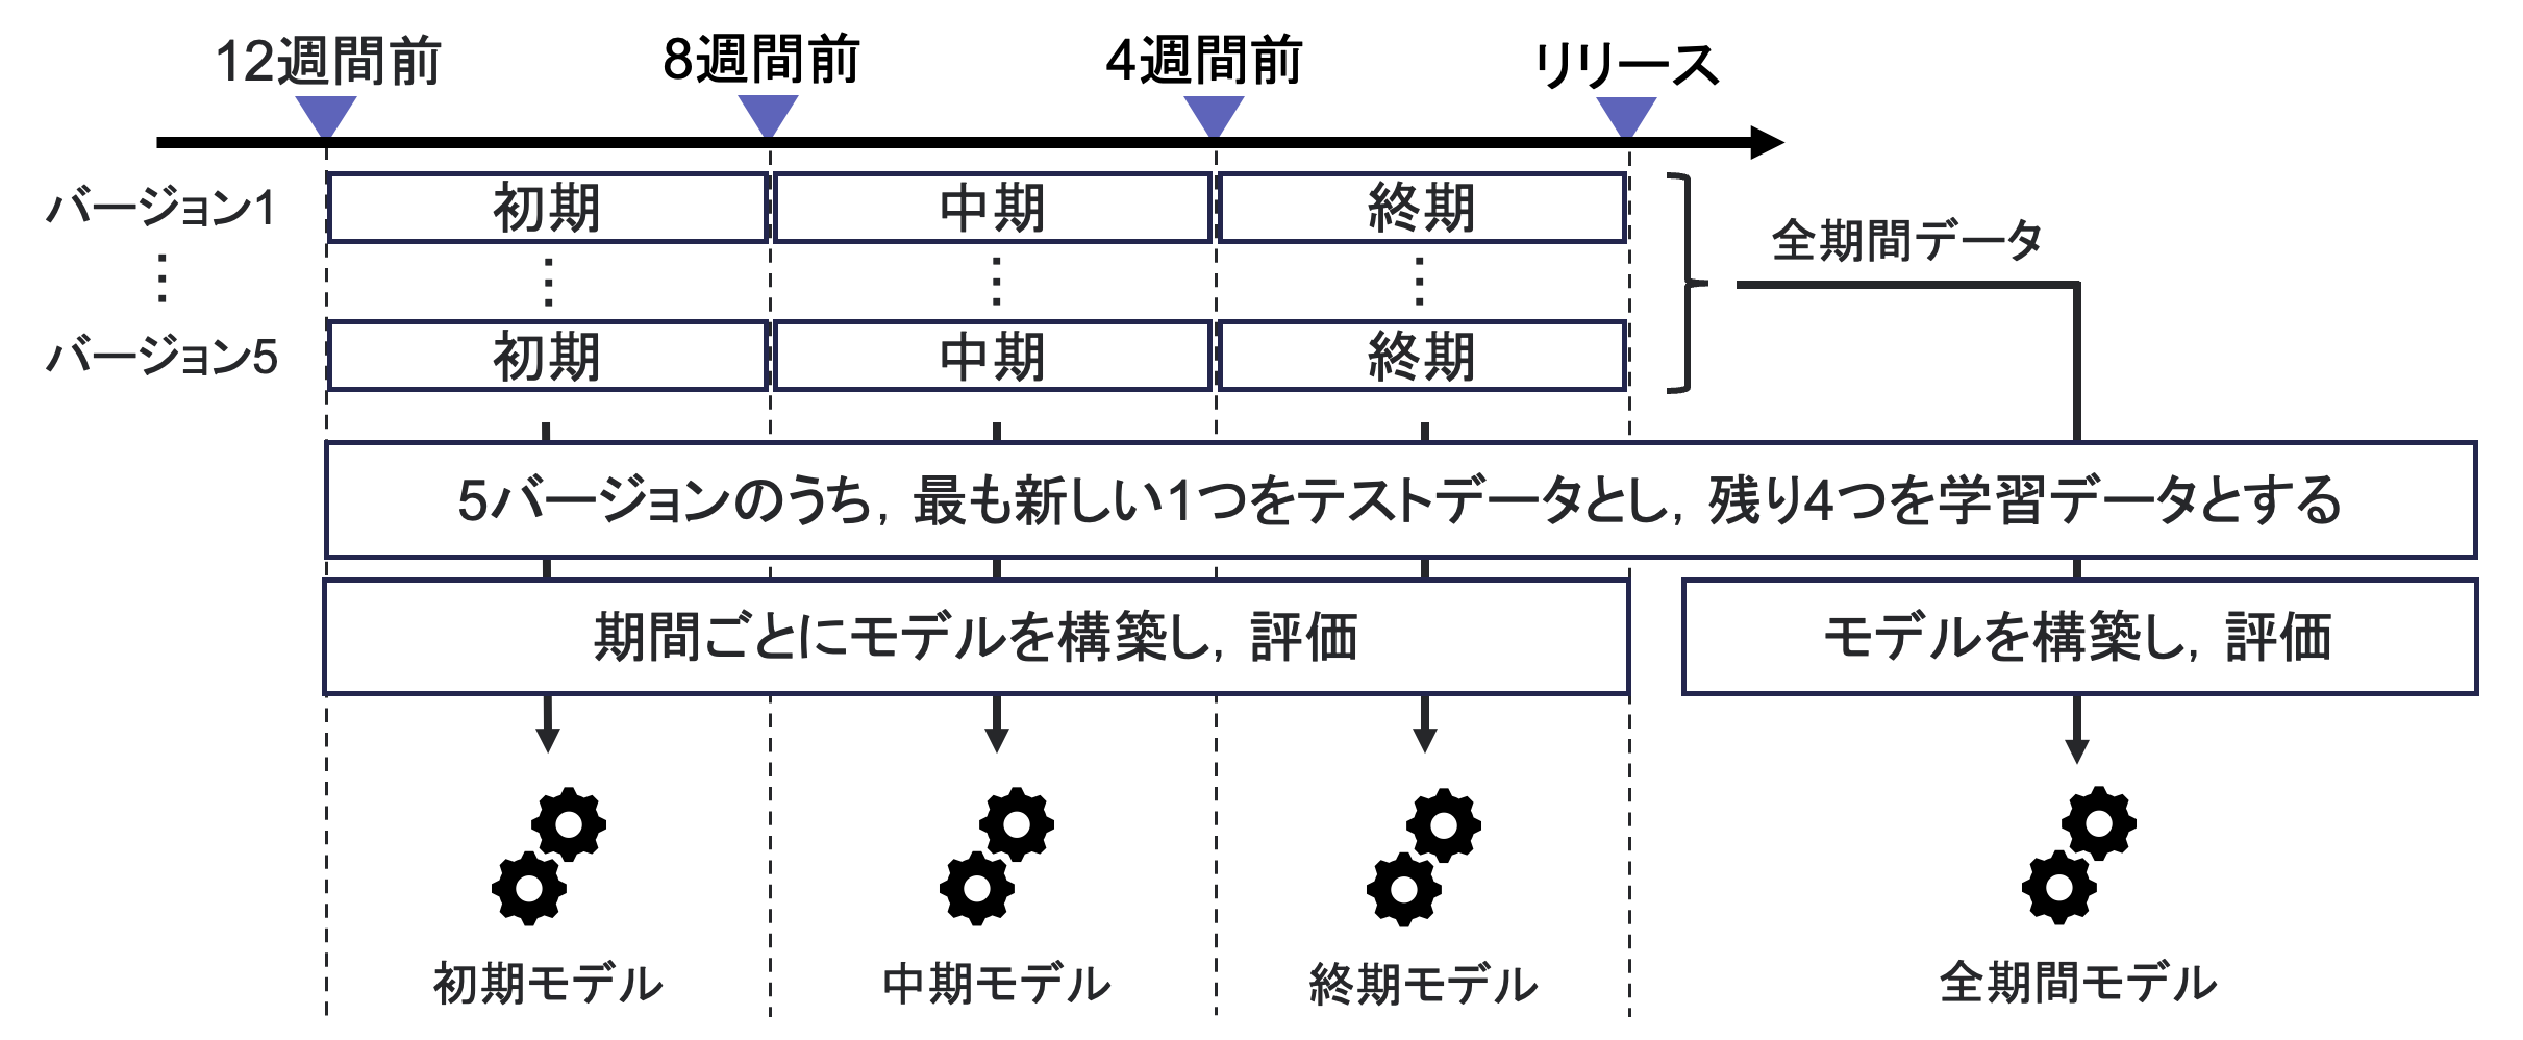
\includegraphics[width=0.8\linewidth]{Uenaka_fig/predict_schematic.pdf}
}
\caption{予測モデル構築の概略図}
\label{fig:predict_schematic}
\end{center}
\end{figure}
%-----------------------

%-------
\begin{table*}[t]
\caption{RQ2-1:検証モデルの予測結果}
\label{table:review_predict}
\centering
  \scalebox{0.87}{

\begin{tabular}{l|cc|cc|cc|cc|cc|cc}
\hline \hline
プロジェクト名               & \multicolumn{6}{c|}{Nova}                                                 & \multicolumn{6}{c}{Neutron}                                              \\ \hline
\multirow{2}{*}{評価指標} & \multicolumn{2}{c|}{初期} & \multicolumn{2}{c|}{中期} & \multicolumn{2}{c|}{終期} & \multicolumn{2}{c|}{初期} & \multicolumn{2}{c|}{中期} & \multicolumn{2}{c}{終期} \\ \cline{2-13}
                      & 提案         & ベース       & 提案         & ベース       & 提案         & ベース       & 提案         & ベース       & 提案         & ベース       & 提案         & ベース       \\ \hline
適合率                   & 0.44       & {\textbf{0.48}}      & 0.56       & {\textbf{0.58}}      & {\textbf{0.56}}       & 0.52      & {\textbf{0.57}}       & {\textbf{0.57}}      & 0.61       & {\textbf{0.64}}      & 0.72       & {\textbf{0.74}}      \\
再現率                   & 0.54       & {\textbf{0.76}}      & 0.52       & {\textbf{0.84}}      & 0.68       & {\textbf{0.78}}      & 0.51       & {\textbf{0.57}}      & 0.55       & {\textbf{0.65}}      & 0.61       & {\textbf{0.66}}      \\
F値                    & 0.48       & {\textbf{0.49}}      & 0.54       & {\textbf{0.69}}      & 0.61       & {\textbf{0.62}}      & 0.53       & {\textbf{0.58}}      & 0.57       & {\textbf{0.65}}      & 0.66       & {\textbf{0.70}}      \\ \hline
プロジェクト名               & \multicolumn{6}{c|}{Cinder}                                               & \multicolumn{6}{c}{Keystone}                                             \\ \hline
適合率                   & {\textbf{0.84}}       & 0.80      & {\textbf{0.89}}       & 0.86      & {\textbf{0.83}}       & 0.79      & {\textbf{0.47}}       & 0.41      & {\textbf{0.63}}       & 0.54      & {\textbf{0.73}}       & 0.67      \\
再現率                   & 0.49       & {\textbf{0.69}}      & 0.57       & {\textbf{0.73}}      & 0.77       & {\textbf{0.81}}      & 0.57       & {\textbf{0.80}}      & 0.38       & {\textbf{0.74}}      & 0.67       & {\textbf{0.81}}      \\
F値                    & 0.62       & {\textbf{0.74}}      & 0.69       & {\textbf{0.79}}      & {\textbf{0.80}}       & {\textbf{0.80}}      & 0.51       & {\textbf{0.54}}      & 0.47       & {\textbf{0.63}}      & 0.70       & {\textbf{0.73}}      \\ \hline
プロジェクト名               & \multicolumn{6}{c|}{Swift}                                                & \multicolumn{6}{c}{Glance}                                               \\ \hline
適合率                   & 0.38       & {\textbf{0.40}}      & {\textbf{0.66}}       & 0.62      & {\textbf{0.66}}       & 0.65      & 0.88       & {\textbf{0.91}}      & 0.68       & {\textbf{0.72}}      & 0.71       & {\textbf{0.75}}      \\
再現率                   & 0.58       & {\textbf{0.71}}      & 0.49       & {\textbf{0.73}}      & {\textbf{0.79}}       & {\textbf{0.79}}      & 0.81       & {\textbf{0.85}}      & 0.78       & {\textbf{0.81}}      & 0.63       & {\textbf{0.71}}      \\
F値                    & 0.46       & {\textbf{0.51}}      & 0.57       & {\textbf{0.67}}      & {\textbf{0.72}}       & 0.71      & 0.85       & {\textbf{0.87}}      & 0.73       & {\textbf{0.76}}      & 0.67       & {\textbf{0.73}}     \\ \hline
\end{tabular}
}

\vspace{4mm}

\caption{RQ2-2:導入モデルの予測結果}
\label{table:merge_predict}
\centering
  \scalebox{0.87}{

\begin{tabular}{l|cc|cc|cc|cc|cc|cc}
\hline \hline
プロジェクト名               & \multicolumn{6}{c|}{Nova}                                                 & \multicolumn{6}{c}{Neutron}                                              \\ \hline
\multirow{2}{*}{評価指標} & \multicolumn{2}{c|}{初期} & \multicolumn{2}{c|}{中期} & \multicolumn{2}{c|}{終期} & \multicolumn{2}{c|}{初期} & \multicolumn{2}{c|}{中期} & \multicolumn{2}{c}{終期} \\ \cline{2-13}
                      & 提案         & ベース       & 提案         & ベース       & 提案         & ベース       & 提案         & ベース       & 提案         & ベース       & 提案         & ベース       \\ \hline
適合率                   & 0.15       & {\textbf{0.18}}      & 0.27       & {\textbf{0.29}}      & 0.31       & {\textbf{0.32}}      & {\textbf{0.27}}       & {\textbf{0.27}}      & {\textbf{0.38}}       & 0.34      & 0.28       & {\textbf{0.30}}      \\
再現率                   & {\textbf{0.74}}       & 0.62      & {\textbf{0.73}}       & 0.64      & 0.52       & {\textbf{0.56}}      & 0.44       & {\textbf{0.52}}      & {\textbf{0.69}}       & {\textbf{0.69}}      & {\textbf{0.55}}       & {\textbf{0.55}}      \\
F値                    & 0.26       & {\textbf{0.27}}      & {\textbf{0.40}}       & {\textbf{0.40}}      & 0.39       & {\textbf{0.41}}      & 0.33       & {\textbf{0.36}}      & {\textbf{0.49}}       & 0.46      & 0.37       & {\textbf{0.39}}      \\ \hline
プロジェクト名               & \multicolumn{6}{c|}{Cinder}                                               & \multicolumn{6}{c}{Keystone}                                             \\ \hline
適合率                   & 0.09       & {\textbf{0.13}}      & 0.26       & {\textbf{0.27}}      & {\textbf{0.39}}       & 0.34      & {\textbf{0.26}}       & {\textbf{0.26}}      & {\textbf{0.37}}       & 0.33      & 0.39       & {\textbf{0.44}}      \\
再現率                   & 0.33       & {\textbf{0.73}}      & 0.54       & {\textbf{0.62}}      & {\textbf{0.57}}       & {\textbf{0.57}}      & {\textbf{0.60}}       & 0.53      & 0.31       & {\textbf{0.54}}      & 0.25       & {\textbf{0.55}}      \\
F値                    & 0.15       & {\textbf{0.22}}      & 0.35       & {\textbf{0.38}}      & {\textbf{0.46}}       & 0.43      & {\textbf{0.36}}       & 0.35      & 0.34       & {\textbf{0.41}}      & 0.30       & {\textbf{0.49}}      \\ \hline
プロジェクト名               & \multicolumn{6}{c|}{Swift}                                                & \multicolumn{6}{c}{Glance}                                               \\ \hline
適合率                   & {\textbf{0.36}}       & 0.30      & 0.12       & {\textbf{0.17}}      & {\textbf{0.16}}       & {\textbf{0.16}}      & {\textbf{0.20}}       & 0.19      & 0.22       & {\textbf{0.27}}      & {\textbf{0.31}}       & 0.24      \\
再現率                   & 0.59       & {\textbf{0.67}}      & 0.19       & {\textbf{0.44}}      & 0.24       & {\textbf{0.32}}      & {\textbf{0.66}}       & 0.55      & 0.57       & {\textbf{0.70}}      & {\textbf{0.81}}       & 0.71      \\
F値                    & {\textbf{0.44}}       & 0.41      & 0.15       & {\textbf{0.25}}      & 0.19       & {\textbf{0.21}}      & {\textbf{0.31}}       & 0.28      & 0.32       & {\textbf{0.39}}      & {\textbf{0.45}}       & 0.36     \\ \hline
\end{tabular}

}
\end{table*}
%-------

\subsubsection{予測モデルの評価}
本分析では,それぞれの期間を対象に,評価指標として適合率,再現率,F値を用い,提案手法の予測精度とベースライン手法の予測精度を比較する.評価指標のうち,適合率はモデルが正例(検証するまたは導入する)と予測したうちの正解割合,再現率は正解のうちモデルが正例と予測した割合であり,この2つの指標はトレードオフの関係である.本研究では,ベースライン手法は期間を問わない汎用性の高いモデルが構築される一方,提案手法は学習するデータをリリースまでの期間で区切っているため,その期間に特化したモデルが構築されると考える.従って,提案手法では再現率よりも適合率が高くなると考え,適合率および適合率と再現率の調和平均であるF値を対象に予測結果を解釈する.

\subsection{結果}
表\ref{table:review_predict}は検証予測モデル,表\ref{table:merge_predict}は導入予測モデルの結果を示す.それぞれ,提案手法とベースライン手法を比較して精度の高いモデルを太字で表記する.

\textbf{(RQ2-1 検証)} 表\ref{table:review_predict}の結果から,提案手法とベースライン手法の精度を比較すると提案手法とベースライン手法の適合率およびF値の差は一部を除き10\%未満であるため,各手法の精度に大きな差は見られなかった.そこで,5.3節において提案手法とベースライン手法で,検証されたチケットと非検証されたチケットを正しく判別できた数を比較することで,各手法の違いを分析する.

\textbf{(RQ2-2 導入)} 表\ref{table:merge_predict}の結果から,提案手法とベースライン手法の精度を比較するとRQ2-1と同じく,提案手法とベースライン手法の適合率およびF値の差は一部を除き10\%未満に止まっているため,各手法の精度に大きな差は見られなかった.そのため,RQ2-1同様,5.3節において提案手法とベースライン手法で,導入されたチケットと非導入されたチケットを正しく判別できた数を比較することで,各手法の違いを分析する.


\subsection{誤判別されたチケットの分析}
本節では,直近のリリースまでの時間に応じて,優先的に検証,または導入されるチケットを特定する本提案手法が,特定可能なチケットの特徴を分析する.具体的には,各モデルにおいて偽陰性(正例データを誤って負例と予測)および偽陽性(負例データを誤って正例と予測)となったチケット数を分析する.

%---------------------
\begin{table*}[]
\caption{提案手法およびベースライン手法のそれぞれで正しく検証/非検証を判別したチケット数}
\label{table:review_predict_contents}
\centering
\scalebox{0.74}{
\begin{tabular}{l|l|c|c|c|cc|cc|cc|cc}
\hline \hline
\multicolumn{1}{c|}{\multirow{3}{*}{プロジェクト}} & \multicolumn{1}{c|}{\multirow{3}{*}{正解ラベル}} & \multicolumn{1}{c|}{\multirow{3}{*}{データ数}} & \multicolumn{1}{c|}{\multirow{3}{*}{両手法で正解}} & \multicolumn{1}{c|}{\multirow{3}{*}{両手法で不正解}} & \multicolumn{8}{c}{片方の手法のみ正解}                                                                     \\ \cline{6-13}
\multicolumn{1}{c|}{}                        & \multicolumn{1}{c|}{}                       & \multicolumn{1}{c|}{}                      & \multicolumn{1}{c|}{}                        & \multicolumn{1}{c|}{}                         & \multicolumn{2}{c|}{初期} & \multicolumn{2}{c|}{中期} & \multicolumn{2}{c|}{終期} & \multicolumn{2}{c}{合計} \\ \cline{6-13}
\multicolumn{1}{c|}{}                        & \multicolumn{1}{c|}{}                       & \multicolumn{1}{c|}{}                      & \multicolumn{1}{c|}{}                        & \multicolumn{1}{c|}{}                         & 提案        & ベース        & 提案        & ベース        & 提案        & ベース        & 提案         & ベース       \\ \hline
\multirow{2}{*}{Nova}                       & 正例                                         & 605                                       & 327                                         & 98                                           & 6         & 42         & 6         & 82         & 12        & 32         & 24         & {\textbf{156}}       \\
                                            & 負例                                         & 634                                       & 157                                         & 272                                          & 39        & 16         & 66        & 22         & 50        & 12         & {\textbf{155}}        & 50        \\ \hline
\multirow{2}{*}{Neutron}                    & 正例                                         & 298                                       & 149                                         & 88                                           & 3         & 9          & 7         & 16         & 9         & 17         & 19         & {\textbf{42}}        \\
                                            & 負例                                         & 184                                       & 71                                          & 77                                           & 10        & 6          & 5         & 4          & 5         & 6          & {\textbf{20}}         & 16        \\ \hline
\multirow{2}{*}{Cinder}                     & 正例                                         & 420                                       & 232                                         & 86                                           & 5         & 34         & 8         & 31         & 9         & 15         & 22         & {\textbf{80}}        \\
                                            & 負例                                         & 113                                       & 40                                          & 41                                           & 12        & 1          & 8         & 1          & 9         & 1          & {\textbf{29}}         & 3         \\ \hline
\multirow{2}{*}{Keystone}                   & 正例                                         & 168                                       & 84                                          & 29                                           & 2         & 13         & 1         & 22         & 4         & 13         & 7          & {\textbf{48}}        \\
                                            & 負例                                         & 147                                       & 28                                          & 54                                           & 24        & 0          & 24        & 1          & 13        & 3          & {\textbf{61}}         & 4         \\ \hline
\multirow{2}{*}{Swift}                      & 正例                                         & 187                                       & 104                                         & 35                                           & 2         & 7          & 4         & 23         & 6         & 6          & 12         & {\textbf{36}}        \\
                                            & 負例                                         & 176                                       & 59                                          & 72                                           & 12        & 8          & 16        & 0          & 5         & 4          & {\textbf{33}}         & 12        \\ \hline
\multirow{2}{*}{Glance}                     & 正例                                         & 165                                       & 116                                         & 22                                           & 6         & 9          & 1         & 2          & 3         & 6          & 10         & {\textbf{17}}        \\
                                            & 負例                                         & 56                                        & 20                                          & 25                                           & 0         & 2          & 1         & 3          & 2         & 3          & 3          & {\textbf{8}}     \\ \hline   
\end{tabular}}

\vspace{4mm}

\caption{提案手法およびベースライン手法のそれぞれで正しく導入/非導入を判別したチケット数}
\label{table:merge_predict_contents}
\centering
\scalebox{0.74}{
\begin{tabular}{l|l|c|c|c|cc|cc|cc|cc}
\hline \hline
\multicolumn{1}{c|}{\multirow{3}{*}{プロジェクト}} & \multicolumn{1}{c|}{\multirow{3}{*}{正解ラベル}} & \multicolumn{1}{c|}{\multirow{3}{*}{データ数}} & \multicolumn{1}{c|}{\multirow{3}{*}{両手法で正解}} & \multicolumn{1}{c|}{\multirow{3}{*}{両手法で不正解}} & \multicolumn{8}{c}{片方の手法のみ正解}                                                                     \\ \cline{6-13}
\multicolumn{1}{c|}{}                        & \multicolumn{1}{c|}{}                       & \multicolumn{1}{c|}{}                      & \multicolumn{1}{c|}{}                        & \multicolumn{1}{c|}{}                         & \multicolumn{2}{c|}{初期} & \multicolumn{2}{c|}{中期} & \multicolumn{2}{c|}{終期} & \multicolumn{2}{c}{合計} \\ \cline{6-13}
\multicolumn{1}{c|}{}                        & \multicolumn{1}{c|}{}                       & \multicolumn{1}{c|}{}                      & \multicolumn{1}{c|}{}                        & \multicolumn{1}{c|}{}                         & 提案        & ベース        & 提案        & ベース        & 提案        & ベース        & 提案         & ベース       \\ \hline
\multirow{2}{*}{Nova}                       & 正例                                         & 358                                       & 178                                         & 92                                           & 14        & 6          & 25        & 12         & 13        & 18         & {\textbf{52}}         & 36        \\
                                            & 負例                                         & 1,540                                     & 677                                         & 439                                          & 52        & 128        & 43        & 97         & 52        & 52         & 147        & {\textbf{277}}       \\  \hline
\multirow{2}{*}{Neutron}                    & 正例                                         & 165                                       & 81                                          & 58                                           & 3         & 7          & 3         & 3          & 5         & 5          & 11         & {\textbf{15}}        \\
                                            & 負例                                         & 501                                       & 245                                         & 170                                          & 18        & 9          & 19        & 9          & 11        & 20         & {\textbf{48}}         & 38        \\ \hline
\multirow{2}{*}{Cinder}                     & 正例                                         & 193                                       & 87                                          & 60                                           & 0         & 12         & 7         & 13         & 7         & 7          & 14         & {\textbf{32}}        \\
                                            & 負例                                         & 727                                       & 306                                         & 236                                          & 66        & 14         & 39        & 29         & 27        & 10         & {\textbf{132}}        & 53        \\  \hline
\multirow{2}{*}{Keystone}                   & 正例                                         & 159                                       & 44                                          & 59                                           & 5         & 2          & 4         & 16         & 5         & 24         & 14         & {\textbf{42}}        \\
                                            & 負例                                         & 349                                       & 147                                         & 91                                           & 12        & 23         & 38        & 8          & 25        & 5          & {\textbf{75}}         & 36        \\ \hline
\multirow{2}{*}{Swift}                      & 正例                                         & 93                                        & 22                                          & 42                                           & 3         & 5          & 1         & 9          & 4         & 7          & 8          & {\textbf{21}}        \\
                                            & 負例                                         & 384                                       & 176                                         & 75                                           & 27        & 14         & 37        & 13         & 29        & 13         & {\textbf{93}}         & 40        \\  \hline
\multirow{2}{*}{Glance}                     & 正例                                         & 73                                        & 38                                          & 15                                           & 5         & 2          & 1         & 4          & 5         & 3          & {\textbf{11}}         & 9         \\
                                            & 負例                                         & 272                                       & 80                                          & 124                                          & 14        & 20         & 6         & 8          & 15        & 5          & {\textbf{35}}         & 33   \\  \hline    
\end{tabular}}
\end{table*}
%---------------------

表\ref{table:review_predict_contents}は,提案手法およびベースライン手法のそれぞれで正しく検証/非検証を判別したチケット数を示す.Novaプロジェクトを対象とした検証予測モデルでは,正例605チケットの中で両モデルで正しく判別できたのは327チケット,誤判別したのは98チケットであった.また,提案手法のみで正しく判別できたのは24チケット(初期で6チケット,中期で6チケット,終期で12チケット)であり,ベースライン手法のみで正しく判別できたのは156チケット(初期で42チケット,中期で82チケット,終期で32チケット)であったことを示す.
表\ref{table:review_predict_contents}から,全てのプロジェクトにおいて,ベースライン手法が提案手法より多くの正例のチケットを正しく判別する一方,負例のチケットは,Glanceプロジェクトを除く5プロジェクトにおいて提案手法がベースライン手法より正しく判別できた.

また,表\ref{table:merge_predict_contents}は,提案手法およびベースライン手法のそれぞれで正しく導入/非導入を判別したチケット数を示す.表\ref{table:merge_predict_contents}から,Nova,Glanceプロジェクトを除く4プロジェクトにおいて,ベースライン手法が提案手法より正例のチケットを正しく判別する一方,負例のチケットはNovaプロジェクトを除く5プロジェクトで提案手法の方がベースライン手法より正しく判別した.

これらの結果から,検証予測/導入予測のいずれも提案手法は負例(検証されないチケット,または導入されないチケット)を検出するために有用なモデルであり,ベースライン手法は正例(検証されるチケット,または導入されるチケット)を検出するために有用なモデルである.このことから,ベースライン手法はリリースまでの期間全体を通して優先されるチケットの特定に有用である一方で,提案手法は一部の期間のみで優先されるチケットの特定に有用であると示唆される.


%%%%%%%%%%%%%%%%%%%%%%
\section{考察}\label{sec:disc}
%%%%%%%%%%%%%%%%%%%%%%

\subsection{優先的に検証/導入されるチケットの特徴が変化するタイミング}\label{secsec:glance_review}
本研究では,各プロジェクトにおけるリリース直前の3ヶ月に導入されたチケット数の上位5バージョンを分析対象として2つのRQを検証した.その結果,リリースまでの期間に応じた検証/導入されるチケットの特徴の違い,およびリリースまでの期間ごとの提案手法の予測精度を明らかにした.これらの結果はプロジェクトによって異なる.RQ2-2では,Neutronプロジェクトでは中期に予測精度が向上する一方で,Glanceプロジェクトでは終期に予測精度が向上している.したがって,今後は優先的に検証,または導入するチケットの特徴が変わる時点を見積もる手法を確立する.

\subsection{妥当性の脅威}
\subsubsection{内的妥当性}
本研究で取り扱う検証予測モデルは,優先的にコードレビューされるチケットを特定することを目的としており,一度検証されたチケットは「検証開始済み」と分類し,次の期間以降から分析対象外としている.しかし,実装者が検証者からの修正要求に基づき改修したソースコードを再提出する場合,検証者は改めて優先して検証するチケットを選択していることが示唆される.今後の研究では,提出時点の優先順位だけでなく,再提出された時点のチケットの優先順位も検討する.

本研究では従来研究で使用された説明変数に基づき7種類の特徴量を分析しているが,今後は変更されたソースコードの変更量だけでなく,内容に関する特徴量(複雑度,等)も分析する.

\subsubsection{外的妥当性}
本研究では,ケーススタディとしてOpenStackプロジェクトのコアコンポーネント6プロジェクトのコードレビューチケットを対象とした.対象とするプロジェクトやリリースバージョンを変更した場合に分析結果および予測精度が変化することが示唆される.しかし,本研究ではGerritを利用するプロジェクトの中でもコードレビューチケットが多く提案されているOpenStackプロジェクトのコアコンポーネントプロジェクトを対象としている.また,その中でも導入されたチケットの多いバージョンを対象としている.そのため,データセットとするプロジェクトやリリースバージョンの変更による分析結果および予測精度への影響は低いと示唆する.

%%%%%%%%%%%%%%%%%%%%%%
\section{おわりに}\label{sec:fig-tab-exp}
%%%%%%%%%%%%%%%%%%%%%%
本論文では,リリースまでの期間に応じて優先的に検証/導入されるコードレビューチケットの特徴の分析を目的に,2つのRQを検証した.データセットとして,OpenStackプロジェクトのコアコンポーネント6プロジェクト(Nova,Neutron,Cinder,Keystone,Swift,Glance)を分析対象とし,チケットの特徴量を収集,比較することで,リリースまでの期間に応じて優先的に検証/導入されるチケットの特徴が異なることを明らかにした.また,それらの特徴量を学習させることで,直近のバージョンリリースに向けて検証される変更提案や導入される変更提案の予測モデルを構築した.モデルの予測精度を評価した結果,提案手法とベースライン手法の精度に大きな差は見られなかった.
また,考察した結果から提案手法は負例(優先的に検証/導入する必要のないチケット)を正確に検出できることが明らかとなった.今後は,優先的に検証,または導入するチケットの特徴が変わる時点を見積もる手法を確立する.

%\textbf{謝辞}\
%本フォーマットの基になったスタイルファイルを作成してくださった方々に感謝します.

%\begin{adjustvboxheight} % needed only when Appendix follows
%\bibliographystyle{jssst}
%\bibliography{sample}
%\end{adjustvboxheight} % needed only when Appendix follows

%以下は付録の例です.必要ならコメントアウトして使用してください.
%なお,その際には参考文献の前後にある adjustvboxheight 環境のコメントアウトを解除してください.
%\appendix
%\section{付録A} 
%これは付録の例です.

%\bibliographystyle{jssst}
\bibliographystyle{plain}
\bibliography{Uenaka_FOSE}

\end{document}